\documentclass[letterpaper,10pt]{article}
\usepackage[top=2cm, bottom=1.5cm, left=1cm, right=1cm]{geometry}
\usepackage{amsmath, amssymb, amsthm,graphicx}
\usepackage{fancyhdr}
\pagestyle{fancy}

\lhead{\today}
\chead{QE Assignment 8}
\rhead{Justin Hood}

\newcommand{\Z}{\mathbb{Z}}
\newcommand{\Q}{\mathbb{Q}}
\newcommand{\R}{\mathbb{R}}
\newcommand{\C}{\mathbb{C}}
\newtheorem{lem}{Lemma}

\begin{document}
\begin{enumerate}
\item See attached Word document.
\item See attached Word document.
\item We consider the Carbon Fiber data from the assignment file.
\begin{enumerate}
\item First, we construct the control charts for $\bar{x}$ and $R$. These charts follow,
\begin{center}
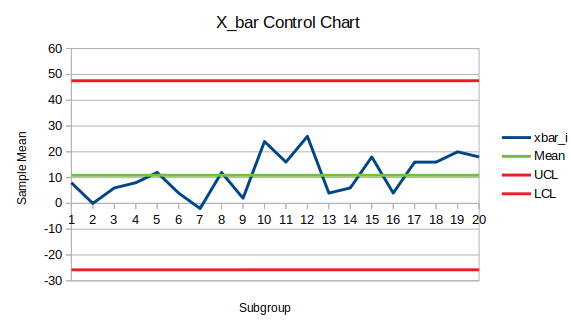
\includegraphics[scale=.75]{3xbarr.png}
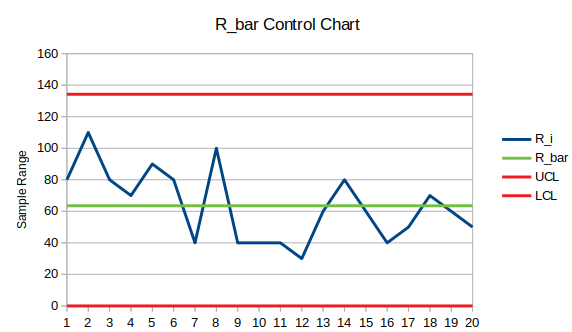
\includegraphics[scale=.75]{3rbar.png}
\end{center}
Here, we see that the process values fall within the UCL and LCL values for both the $\bar{x}$ and $R$ values. Aside from a possible gentle slope in the data, it appears to be performing within acceptable values, with fairly random variation point to point. So, we conclude that the process is likely in control.
\item Next, we perform the same analysis on the standard deviation values. The results follow,
\begin{center}
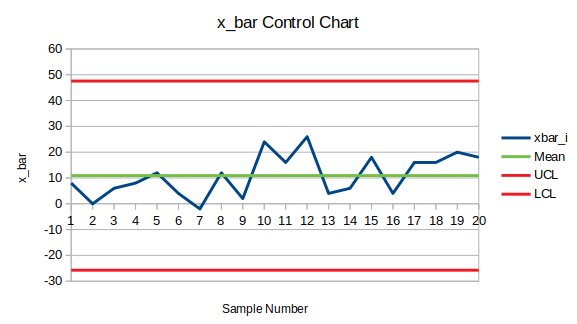
\includegraphics[scale=.75]{3xbars.png}
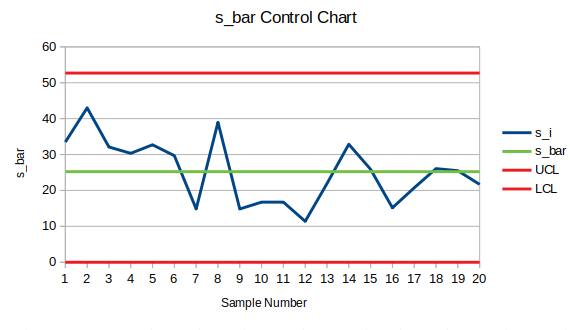
\includegraphics[scale=.75]{3sbar.png}
\end{center}
Here, we see that the process values fall within the UCL and LCL values for both the $\bar{x}$ and $s$ values. Aside from a possible gentle slope in the data, it appears to be performing within acceptable values, with fairly random variation point to point. So, we conclude that it is likely in control.
\end{enumerate}
\item We now consider the printed circuit board data. Again, we compute the $\bar{x}$ and $R$ charts for the data, they follow,
\begin{center}
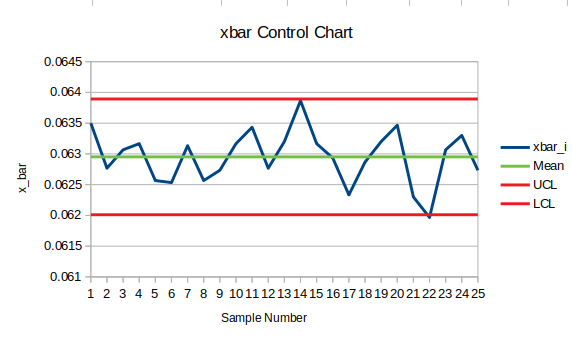
\includegraphics[scale=.75]{4xbar.png}
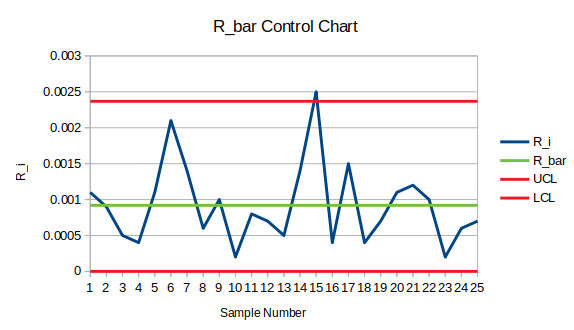
\includegraphics[scale=.75]{4rbar.png}
\end{center}
In this example, we see that the data has much more variance across sample. While almost all of the data falls within the bounds we have computed, we see that there are a few data points that fall on or over the boundary. Thus, we conclude that the data is somewhat outside of control. The process merits further analysis into improving the results in some way.
\item Finally, we consider the hospital data. Again, we compute the control charts for $\bar{x}$ and $R$.
\begin{center}
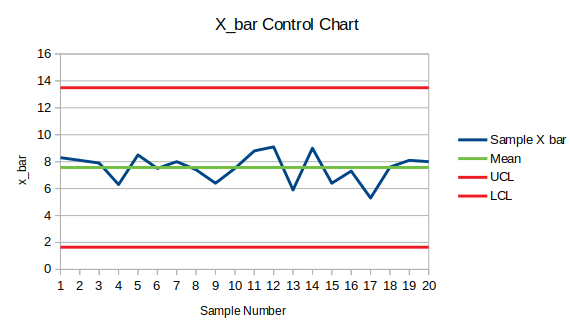
\includegraphics[scale=.75]{5xbar.png}
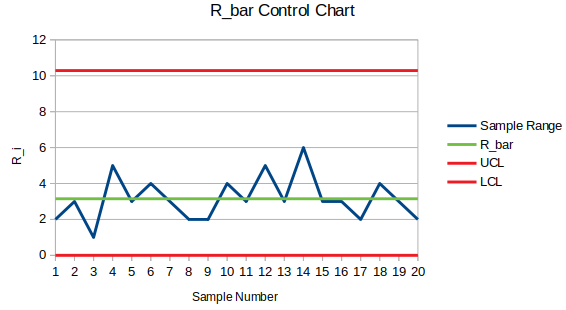
\includegraphics[scale=.75]{5rbar.png}
\end{center}
Here, we see that the data is falling well within the predicted limits, with random variation sample to sample. We conclude that the wait time is within SPC control limits. 
\end{enumerate}
\end{document}
